\section{Příklad 4}
% Jako parametr zadejte skupinu (A-H)
\ctvrtyZadani{H}
\begin{figure}[H]
    \centering
    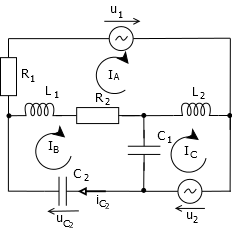
\includegraphics[scale=0.8]{pic4/Pr4_2022.png}
    \caption{Smyčkové proudy}
\end{figure}
U střídavého napětí využijeme stejné ohmovy zákony jako jsme využívali dosud. Jen s rozdílem, že nám zde přibyli impedance nelineárních součástek. Pro metodu smyčkových využijeme matici podobně jako v příkladu 3 jen se změnou, že nyní počítáme proudy smyček narozdíl od uzlových napětí.

Impedance pro cívku a kondenzátor spočteme následovně:
\begin{align*}
	\omega &= 2\pi f \\
	\Z{C} &= \frac{-j}{\omega C}\\
	\Z{L} &=  j\omega L
\end{align*}

\begin{align*}
	\I{A}:\quad&\Uu{1} + \Uu{R1} + \Uu{L2} + \Uu{R2} + \Uu{L1}  = 0\\
	\I{B}:\quad&\Uu{L1} + \Uu{R2} + \Uu{C2} + \Uu{C1} = 0 \\
	\I{C}:\quad&\Uu{L2} + \Uu{2} + \Uu{C1}  = 0
\end{align*}

\begin{align*}
	\I{A}:\quad&\I{A}(\Z{L1}+\Z{L2}+\R{1}+\R{2}) - \I{B}(\Z{L1}+\R{2}) - \I{C}\Z{L2} = -\Uu{1} \\
	\I{B}:\quad&-\I{A}(\Z{L1} + \R{2}) + \I{B}(\R{2}+\Z{L1}+\Z{C1}+\Z{C2})-\I{C}\Z{C1} = 0 \\
	\I{C}:\quad&-\I{A}\Z{L2} - \I{B}\Z{C1} + \I{C}(\Z{C1}+\Z{L2}) = -\Uu{2}
\end{align*}

Matice pro proudové smyčky:
	
\begin{align*}
	\begin{pmatrix}
		Z_{L2}+Z_{L1}+R_1+R_2&-Z_{L1}-R_2&-Z_{L2}\\ 
		-Z_{L1}-R_2&R_2+Z_{L1}+Z_{C1}+Z_{C2}&-Z_{C1}\\ 
		-Z_{L2}&-Z_{C1}&Z_{C1}+Z_{L2}
	\end{pmatrix}
	\times
	\begin{pmatrix}
		I_A\\ I_B\\ I_C
	\end{pmatrix}
	=
	\begin{pmatrix}
		-U_1\\ 0\\ -U_2
	\end{pmatrix}
\end{align*}

\subsection{Výpočet napětí a fázového posunu \Ll{2}}
Pro výpočet \Uu{C2} využijeme Ohmův zákon. Nesmíme zapomenout že se zde pracujeme s množinou imaginárních čísel, takže pro náš výsledek musíme využít vzorec pro absolutní hodnotu imaginárního čísla:

\begin{align*}
	\Uu{C2} &= \I{B}\times j\omega \Cc{2} \\
	\Uu{C2}| &= \sqrt{Re(\Uu{C2})^2 + Im(\Uu{C2})^2}
\end{align*}

Fázový posun vypočítáme jako arkus tangens, kde x je reálná část imaginárního čísla a y je imaginární část imaginárního čísla.

\begin{align*}
	\varphi_{C2}&= arctan(\frac{Im(\Uu{C2})}{Re(\Uu{C2})})
\end{align*}

\subsection{Dosazení}
Impedance:

\begin{align*}
	\omega &= 2\pi f \\
	\Z{C1} &= \frac{-j}{\omega \Cc{1}}\\
	\Z{C2} &= \frac{-j}{\omega \Cc{2}}\\
	\Z{L1} &=  j\omega \Ll{1} \\
	\Z{L2} &=  j\omega \Ll{2}
\end{align*}


\begin{align*}
\begin{pmatrix}20+95.5016*j+44.766375*j	&-10-95.5016*j&-44.766375*j\\ 
-10-95.5016*j&10+95.5016*j-10.8088*j-23.93378*j&10.8088*j\\ 
-44.766375*j&10.8088*j&44.766375*j-10.8088*j
\end{pmatrix}
\begin{pmatrix}I_A\\ 
I_B\\ 
I_C
\end{pmatrix}
=
\begin{pmatrix}
-5\\ 
0\\ 
-6
\end{pmatrix}
\end{align*}

\begin{align*}
	\I{A} &= (-0,0979-0,27j)\ \si{\ampere} \\
	\I{B} &= (-0,1128-0,4187j)\ \si{\ampere} \\
	\I{C} &= (-0,0931-0,046j)\ \si{\ampere}
\end{align*}

\begin{align*}
	\I{C2} &= \I{B} = (-0,1128-0,4187j)\ \si{\ampere} \\
	\Uu{C2} &= \I{C2} \times \Z{C2} = (-10,02107+2,69973j)\ \si{\volt} \\
	\varphi_{C2}&= \arctan(\frac{Im(\Uu{C2})}{Re(\Uu{C2})}) = \arctan\frac{2,69973}{-10,37837} =-0,254491 rad = 165,41874^\circ \\
	|\Uu{C2}| &= \sqrt{Re(\Uu{C2})^2 + Im(\Uu{C2})^2} = \sqrt{(-10,02107)^2+2,69973^2} = 10,37837\ \si{\volt}
\end{align*}